\section{Background and Objectives}\label{sec:bg}

\begin{table*}[]
\centering
\begin{tabular}{|l|l|l|l|l|}
\hline
 & \textbf{Trigger-based} & \textbf{Driver functions} & \textbf{Orchestrators} & \textbf{\name{}} \\ \hline
\textit{Purely Serverless}          & \cmark & \cmark & \xmark & \cmark \\ \hline
\textit{Higher-level interface}     & \xmark & \xmark & \cmark & \cmark \\ \hline
\textit{Exactly-once semantics} & \xmark & \xmark & \cmark & \cmark \\ \hline
\textit{Pay-for-what-you-use billing}       & \cmark & \xmark & \cmark & \cmark \\ \hline
\end{tabular}
\caption{Comparison with existing approaches}
\label{table:positioning}
\end{table*}


% Large-scale applications composed of many functions~\cite{excamera, gg-atc,
% deathstar} introduce several new challenges to serverless computing. 

In this section, we describe why it is hard to compose large serverless
workflows, why a purely serverless architecture is interesting and what our
objectives are.

\subsection{Evolution of Serverless Workflows}

\begin{figure}[t!]
    \centering
    \scalebox{.7}{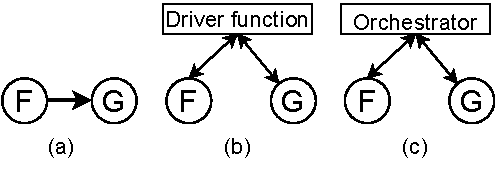
\includegraphics[width=\columnwidth]{figures/ChainExample.pdf}}
    \caption{Chaining two functions with triggers, driver functions and
    orchestrators. In the trigger-based approach, \texttt{F} asynchronously
    invokes \texttt{G} with \texttt{F}'s result. In the driver functions
    approach, a driver function first synchronously invokes \texttt{F},
    usually via HTTP, and after \texttt{F} returns, synchronously invokes
    \texttt{G} with \texttt{F}'s result. Workflow orchestrators provide
    higher-level interfaces (e.g., AWS Step Functions state machines) to
    express function compositions such that \texttt{F}'s code does not contain
    explicit control-flow logic of invoking \texttt{G}. But architecturally,
    orchestrators are similar to driver functions: an orchestrator instance
    invokes \texttt{F}, waits for \texttt{F} to return and then invokes
    \texttt{G} with \texttt{F}'s result.}
    \label{fig:chain-example}
\end{figure}

\subsubsection{Ad-hoc composition: triggers and driver functions}

The original serverless abstraction is designed around developing individual
functions--a \textit{single} unit of work that can run independently on any
machine. However, this design does not provide a higher-level interface to
easily express control-flow logic \emph{between} functions. To build larger
applications that are composed from multiple functions, early adopters use
function invocation APIs to exress control-flows in an ad-hoc manner in one of
the following two ways: \textit{ i. trigger-based}
composition~\cite{netherite} where functions invoke their immediate downstream
functions with \emph{asynchronous} triggers, usually via a queue or data
store, (e.g., a lambda writes to an SQS queue or S3 bucket which in turn sends
an event to Lambda and triggers the next function), and \textit{ii.driver
functions}~\cite{beldi} where a single function, similar to the
\texttt{main()} function of a program, encompasses the control-flow logic and
invokes other functions \emph{synchronously}. Figure~\ref{fig:chain-example}
depicts an example of chaining functions with the two approaches.
	
\shadi{shouldn't the first figure (a) have a storage in the middle?}\dhl{For
the figure, I was intentionally not showing a storage because 1. the point is
that it's \emph{asynchronous}, 2. AWS Lambda's async invoke API actually hides
the fact that it's going over a queue. You simply call \texttt{invoke(data,
RequestType=Event)}, and that adds an item to Lambda's internal queue, which
then generates an event that triggers your lambda. I've adjusted the text to
highlight the \emph{asynchronous} nature and downplay the details about
storage. Take a look and let me know if it works. If not, we can add storage
into Figure 1. But my concern with it is that people might think \name{} needs to
manage similar intermediary data stores while in fact it's managed by Lambda.
The important feature we care about is just that the invocation is
asynchronous. We don't actually care that it's going over a storage.}
\shadi{can we add the "async" keyword on the figure. Right now the figure is very simple. Not sure it is worth having the figure at all. It is not adding much more than what is in the text. One option would be to remove the figure entirely and just rely on text. }
\shadi{from the figure and text it is not clear what is the diff between
driver and coordinator. }\dhl{Edited the figure caption. Take a look and let
me know if it's on point and sufficient? High-level note: I think the missing
piece in the text is how the different approaches program differently. How
developers write actual code.} \shadi{The caption is clear but too detailed for a caption. I still don't see much value in the figure unless you can somehow capture the details in the caption in the figure itself. For example, for (a) you can add async on the arrow, for (c) you can add a small box with "app logic" being submitted to the orchestrator depicting the high level API. If this does not make sense, maybe remove the figure?}

\shadi {let's just use trigger based throughout the paper}\dhl{Yes.}





%The original serverless abstraction is designed around individual functions
%and does not provide an interface for programming larger applications with
%many functions. As a result, early adopters use low-level function invocation
%APIs to compose functions in an ad-hoc manner, and there are two primary
%approaches.

%The first approach is called trigger-based or unstructure
%composition~\cite{netherite} where functions invoke each other
%\emph{asynchronously} via storage triggers. The second is called driver
%functions~\cite{beldi} where a single \shadi{driver} function invokes other functions
%\emph{synchronously}. Figure~\ref{fig:chain-example} depicts an example of
%chaining functions with the two approaches. \shadi{shouldn't the first figure (a) have a storage in the middle?} \shadi{from the figure and text it is not clear what is the diff between driver and coordinator. }


Although both approaches are ``purely serverless'', i.e., they do not require
adding additional components to the serverless infrastructure, neither is
well-suited for the complexities of emerging serverless applications that
consists of 10s or 100s of functions~\cite{excamera, hello-retail}.
Trigger-based composition scatters control-flow logic across constituent
functions, thus, development quickly gets unwieldy as the number of functions in the
application increases. More importantly, it does not support all forms of
composition such as fan-in that aggregates results from multiple (potentially)
concurrent functions after \textit{all} are complete \footnote{\shadi{This is due to the asynchronous invocations of triggers with no support for either synchronizing across concurrent
	instances, or the inability to pass caller's data other function's data to the callee.}}.

%, \dhl{as
%asynchronous invocation alone do not support synchronizing across concurrent
%instances and can only pass the caller's data, and not other functions' data,
%to the callee.}

On the other hand, driver functions concentrate control flow in a single
function and support arbitrary composition. However, they can  create ``double
billing'' by the driver function idly waiting for callees to return. Also, the
driver function has to wait until all functions in the application complete,
which risks hitting the commonly imposed timeouts (e.g., 900 second on AWS
Lambda) and limits scalability.


Moreover, neither approach provides the commonly sought-after ``exactly once''
semantics~\cite{netherite, beldi, boki, formal-foundation-exec-gtnee}.
Functions can crash mid-execution due to runtime or hardware faults which may
lead to automatic retries~\cite{aws-lambda-retry, azure-functions-retry}. Even
in the absence of faults, most FaaS systems only ensure at-least-once
execution~\cite{aws-lambda-async-invoke, azure-functions-exec-guarantee}, so a
single invocation can trigger multiple, potentially concurrent, instances.


%\dhl{Maybe explain why fan-in is not supported as a contrast to \name{}. But
%tricky because there's nothing fundamentally stopping unstructured composition
%from achieving fan-in as \name{} also demonstrated. Maybe the main difference
%is ad-hoc vs ..not. Or maybe the main difference is the addition of strongly
%consistent data stores and how we use them.} \shadi{I agree that you should
%say why fan-in is not supported. does the current text handle that?}\dhl{Yes
%but I'm not confident with the current explanation. Please take a look at the
%end of the 3rd to last paragraph. I wrote it in red text.}



%Although both approaches are purely serverless and do not require adding
%additional components to the serverless infrastructure, they each have
%important drawbacks. Unstructured composition scatters control flow across
%constituent functions. As the number of functions increases, development can
%quickly get unwieldy. Moreover, it does not support important composition
%patterns such as fan-in, where we want to invoke a function to aggregate the
%results of multiple upstream functions only after all of them are complete.


%Compared with unstructured composition, driver functions concentrate control
%flow in a single function and supports \shadi{complex patterns such as}aggregation. However, users pay for the
%time when driver functions idly wait for callees to return. This causes
%\emph{double billing}~\cite{double-billing}. \shadi{how about the fact that it is sync? doesn't that add delay, e.g., in a fan-out} Also, serverless platforms
%commonly impose timeouts. A driver function instance has to wait until all
%functions in the application are complete, which risks timeouts and limits
%application scale.

%Moreover, both approaches suffer from weak execution guarantees of the
%underlying serverless system. Functions can crash mid-execution due to runtime
%or hardware faults which may lead to automatic retries~\cite{aws-lambda-retry,
%azure-functions-retry}. Even in the absence of faults, most serverless
%platforms only ensure at-least-once execution~\cite{aws-lambda-async-invoke,
%azure-functions-exec-guarantee} so a single invocation can trigger multiple,
%potentially concurrent, instances. \shadi{if no failures, why would there be multiple invokes?}

\subsubsection{Workflow orchestrators}

To simplify the development of large serverless applications, many workflow
orchestrator have emerged~\cite{excamera, gg-atc, aws-step-functions,
google-cloud-composer, google-workflows, durable-functions}. Orchestrators
are  high-level programming interface running on top of the primitive
functions and hide the low-level complexities of using multiple functions.
They offer a  rich set of composition primitives, such as branching,
chaining, fan-out and fan-in while ensuring exactly-once semantics and
long or no runtime limits.

Orchestrators provide these features by hosting a separate ``orchestration''
service alongside the low-level functions to manage the execution of a
workflow. All functions invocation are initiated by the orchestrator and all
states (e.g., function results) pass through the orchestrator. Similar to
driver functions, for every workflow invocation, an orchestrator instance
invokes a constituent function, waits for its result and passes it to
downstream functions via invocation.

However, adding this additional standalone service creates several important
drawbacks that undermine the key benefits of the serverless abstraction. The
end-to-end performance now depends on both the orchestrator service and the
FaaS engine. A slow orchestrator can become a bottleneck and nullify the
performance and scalability advantages of serverless. Moreover, developing a
fast and scalable orchestrator is a difficult and expensive task that
requires a dedicated engineering team which in turn will increase the cost of
running serverless applications. Running a separate orchestrator service also
requires additional computational resources which translates to cost overheads
and potentially idle-billing. Most importantly, the developers no longer have
any control on how to optimize the performance, scalability, or cost of
orchestrator based environments.   \shadi{should we give a cost comparison
example here? something in the lines of "For example, the pricing schema of
AWS step functions makes running a simple X app Y times more expensive that
running directly on AWS Lambda, and the developers have no control on this
pricing."}


\shadi{" Platform-specific orchestrators force developers to write with
proprietary APIs and locks them in a particular cloud provider." move and
merge into goals or later section}



%Recently, workflow orchestrators have emerged to tackle the challenges of
%large serverless applications~\cite{excamera, gg-atc, aws-step-functions,
%google-cloud-composer, google-workflows, durable-functions}. Orchestrators are
%separate hosted services that execute workflow definitions, invoke constituent
%functions and manage workflow states. Architecturally, they are similar to
%driver functions (Figure~\ref{fig:chain-example}). For every workflow
%invocation, an orchestrator instance invokes a constituent function, waits for
%its result and passes it to downstream functions via invocation. All functions
%invocation are initiated by the orchestrator and all states (e.g., function
%results) pass through the orchestrator.

%Different from ad-hoc composition, orchestrators offer (1). higher-level
%programming interfaces that directly express function interactions and hide
%low-level APIs, (2). a rich set of composition primitives, including
%branching, chaining, fan-out and fan-in, (3). exactly-once semantics for
%workflow execution, and (4). long or no runtime limits.

%While fixing the flaws of ad-hoc composition, the orchestrator design creates
%several important drawbacks that neglect or even compromise key benefits of
%the serverless abstraction: (1). End-to-end performance now also depends on
%the orchestrator service that is separate from the FaaS engine. A slow
%orchestrator can become a bottleneck and nullify the fast autoscale advantage
%of serverless. (2). Serverless computing already offers compute and storage
%building blocks that are highly performant and scalable. Adding yet another
%separate service that is a mixture of compute and storage is repeating the
%difficult and expensive task of developing and maintaining a large-scale system,
%which often requires a dedicated engineering team.(3). Platform-specific
%orchestrators force developers to write with proprietary APIs and locks them
%in a particular cloud provider.\dhl{I'm hesitant to include the 3rd point
%because 1. we can't demonstrate that \name{} solves this problem. 2. while
%it's a benefit, it feels more an engineering problem than a research problem.
%3. FaaS functions are already platform-specific. Lambda, Azure functions, etc.
%all have different propritary APIs.} \shadi{I thought the point here was to be a design goal of "interoperability".}
%\dhl{Yes, but the problem is that current \name{} implementation only works on AWS. So we can't show/prove that we achieved interoperability if we list that as a goal. }

\subsection{Research question and objectives}
In this paper, we examine whether we can have the best of both worlds:
\emph{Can we preserve the advantages of workflow orchestrators while building
entirely on top of the existing serverless computing abstraction (no
supplemental services)?}

Table~\ref{table:positioning} compares the current solutions and \name{}.
Specifically, we aim for a system with the following objectives:

\begin{itemize}

    \item \textbf{Purely serverless: } The system should work within the
    current serverless environment and not require adding any new services.

    The system should execute workflows solely as event-driven serverless
    functions, and use serverless storage, when necessary, to enable stateful
    control-flow patterns (e.g., fan-in).

    \item \textbf{Higher-level API \& support for common interactions}
    Developers should compose functions with high-level primitives similar to
    existing workflow orchestrators instead of ad-hoc mechanisms and be able
    to simply express common control-flow patterns such as chaining,
    branching, fan-out and fan-in.

    \item \textbf{Exactly-once semantics} Even if a function executes multiple
    times, due to retries or duplicate invocations, concurrently or
    non-concurrently, the final state should appear that the execution
    happened only once.

    \item \textbf{Comparable performance and costs} The system should at least
    have comparable costs and performance as the state-of-the-art workflow
    orchestrators. Similarly, it should avoid idle-billing. Users should only pay
    for the resources used rather than idle time wait for other functions to
    return. \shadi{@David: double-billing seems like a minor issue with only
    driver functions. not at the same level of importance as the other goals. I
    merged them into one bullet point. } \dhl{Yes, great point!}

    \shadi{should we call it idle billing throughout the paper instead of
    double billing? It is not exactly double...}\dhl{Yeah, I like "idle
    billing" better. Used "double billing" because of prior work. But if we no
    longer need to mention this problem anywhere else in the paper other than
    the driver functions section, I think we can just define and explain the
    problem and then be done with it.}

\end{itemize}

\shadi{in the table, should we have double billing? maybe another term would
be better?}\dhl{Changed it to pay-for-what-you-use billing}




%In this paper, we examine whether we can have the best of both worlds. We
%argue that it is possible to preserve the advantages of workflow orchestrators
%while building entirely on top of the existing serverless computing
%abstraction without adding any supplemental components.
%
%Specifically, we aim for a system with the following objectives:
%
%\paragraph{\emph{Purely serverless}} The system should work within the current
%serverless environment and not require adding any new services.
%
%The system should execute workflows solely as event-driven serverless
%functions, and use serverless storage, when necessary, to enable stateful
%operations (e.g., fan-in).
%
%\paragraph{Higher-level programming interface} Developers should express
%function compositions with higher-level primitives similar to exising workflow
%orchestrators (e.g., AWS Step Functions) instead of ad-hoc mechanisms.
%
%\paragraph{Supports all common interactions} The system should support all
%composition patterns commonly used in orchestrators today, including chaining,
%branching, fan-out and fan-in.
%
%\paragraph{Exactly-once semantics} Even if a function executes multiple times,
%due to retries or duplicate invocations, concurrently or non-concurrently, the
%final state should appear that the execution happened only once.
%
%\paragraph{Avoids double billing} Users should only pay for the resources
%used. Functions should not synchronously wait for other functions to return.
%
%\paragraph{Comparable performance and costs} The system should at least have
%comparable costs and performance as the state-of-the-art workflow
%orchestrators.

